%---------------------------------------------------------------------------%
\lecture{Research Presentation}{lec_present_result}
%---------------------------------------------------------------------------%
\section{Nonlinear Simulations}
%---------------------------------------------------------------------------%
\begin{frame}[fragile]
    \frametitle{MSTE as DNS Initial Conditions}
    \begin{itemize}
        \item MSTE are equilibria of the quasilinear equations \textbf{not} the full nonlinear equations\newline
        
        \item But they ought to be close to the nonlinear system's strange attractor\newline
        
    \end{itemize}
    % \item MSTE initial conditions:
    \begin{columns}[T]
        \begin{column}{.28\textwidth}
            % \centering 
            \textbf{Linear Initial Conditions}
            \vspace{0.07\linewidth}
            \begin{align}
                T(x, z)\big|_{t=0} &= 0.5 - z + \mathcal{N} \nonumber \\
                \vec{u}(x, z)\big|_{t=0} &= \vec{0} \label{EQ:linear_ic}
            \end{align}            
        \end{column}
        \begin{column}{.28\textwidth}
            % \centering
            \textbf{MSTE Initial Conditions}
            \begin{align}
                T(x, z)\big|_{t=0} &= \overline{T}(z) + \sum_{n=1}^N  A_n \Re \Big[ \theta_n(z) e^{ik_{x_n}x} \Big] + \mathcal{N} \nonumber \\
                \vec{u}(x, z)\big|_{t=0} &= \sum_{n=1}^N A_n \Re \Big[\Big( U_n (z) \hat{x} + W_n(z) \hat{z} \Big) e^{ik_{x_n}x} \Big] \label{EQ:mste_ic}
            \end{align}
        \end{column}
    \end{columns}
\end{frame}


\begin{frame}
    \frametitle{Nonlinear Simulations with MSTE Initial Conditions}
    % \includemedia[
        %                 width=0.3\linewidth,
        %                 height=0.7\linewidth,
        %                 keepaspectratio,
        %                 activate=pageopen,
        %                 playbutton=fancy,
        %                 ]{}{Video/2d_rayleigh_benard_Ra10e8.mp4}
    \begin{center}
        \textbf{No Convective Turnover!}
        \vfill

        {\includemedia[
            width=0.6\linewidth,
            height=0.35\linewidth,
            activate=pageopen,
            playbutton=none,
            ]{}{Video/merged_good_looped.mp4}}        
    \end{center}

\end{frame}
%---------------------------------------------------------------------------%
\begin{frame}[fragile]
    \frametitle{Nonlinear Simulations with MSTE Initial Conditions}
    \begin{itemize}
        \item MSTE simulations do not exhibit characteristic turnover\newline
        
        \item They take longer to equilibrate due to exagerrated flows which viscously attenuate
        
    \end{itemize}
    % \tikzart[t=v,x=9.5,y=-6.5,w=0.5]{Video/2d_rayleigh_benard_Ra10e8.mp4}
    % [\includegraphics{cover_image}]
    % \movie[width=8cm,height=4.5cm]{test}{2d_rayleigh_benard_Ra10e8.mov}
    \begin{columns}[T]
        \begin{column}{.3\textwidth}
            {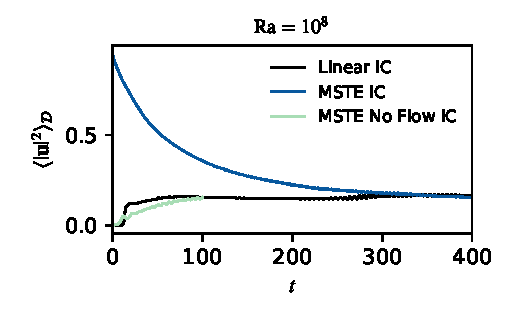
\includegraphics[height=0.75\textwidth]{sim_eq_ke_noflow.pdf}}
        \end{column}
        \begin{column}{.3\textwidth}
            {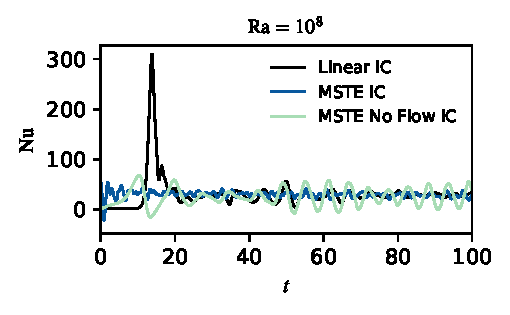
\includegraphics[height=0.75\textwidth]{sim_eq_nu_noflow.pdf}}
        \end{column}
    \end{columns}
\end{frame}
%---------------------------------------------------------------------------%
